\documentclass[tikz,border=0pt]{standalone}
\usepackage{fontspec,unicode-math}
\setmainfont{FiraMath-Regular.otf}[Path=fonts/]
\setmathfont{FiraMath-Regular.otf}[Path=fonts/]
\usepackage{xcolor}
\definecolor{Blue}{HTML}{7188A3}
\definecolor{BlueFill}{HTML}{E5EAF0}
\definecolor{Green}{HTML}{829C8B}
\definecolor{Ink}{HTML}{3B4252}
\definecolor{Grid}{HTML}{D8DCE2}
\definecolor{Panel}{HTML}{F4F5F5}
\begin{document}
\color{Ink}
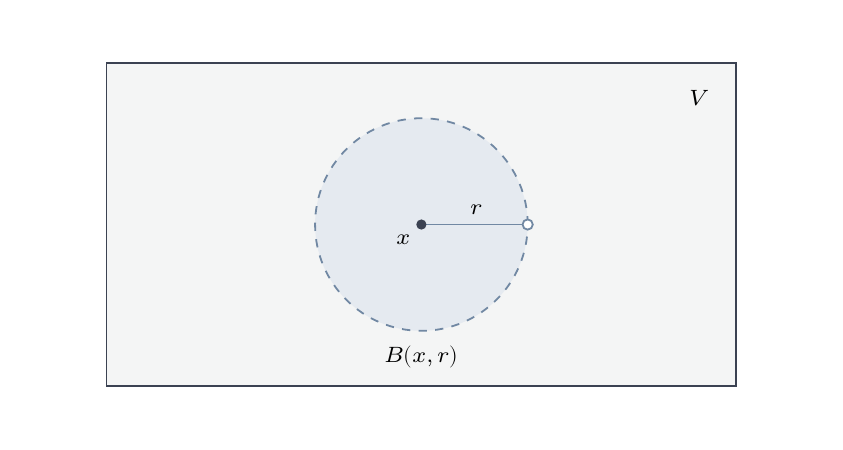
\begin{tikzpicture}[x=10mm,y=10mm,line width=.65pt,font=\fontsize{8}{10}\selectfont]
\path[use as bounding box] (0,0) rectangle (10,5);
\filldraw[fill=Panel,draw=Ink] (1,.45) rectangle (9,4.55);
\node at (8.5,4.1) {$V$};
\fill[BlueFill] (5,2.5) circle[radius=1.35cm];
\draw[Blue,dashed] (5,2.5) circle[radius=1.35cm];
\draw[Blue] (5,2.5)--(6.35,2.5);
\node[above] at (5.7,2.5) {$r$};
\fill[Ink] (5,2.5) circle[radius=.65mm];
\node[below left] at (5,2.5) {$x$};
\filldraw[fill=white,draw=Blue] (6.35,2.5) circle[radius=.65mm];
\node at (5,.82) {$B(x,r)$};
\end{tikzpicture}

\end{document}
